\documentclass{article}
\usepackage[left=0.5in,top=0.5in,right=0.5in,bottom=0.5in]{geometry}
\usepackage[english]{babel}
\usepackage[utf8]{inputenc}
\usepackage[table]{xcolor}
\usepackage{amssymb,amsmath,amsthm}
\usepackage{changepage,threeparttable}
\usepackage{booktabs,multirow}
\usepackage{graphicx}
\usepackage{soul}
\graphicspath{{./images/}}
\def\F#1{\(#1\)}
\title{Lab 9: RC Discharge}
\author{Philip Kim}
\date{\today}
\begin{document}
\maketitle
\vspace*{-1cm}
\begin{table}[!htp]\centering
  \begin{tabular}{|c|c|c|c|c|c|c|c|c|c|c|}\hline
    \multicolumn{11}{|c|}{\textbf{Table 1: Discharge}} \\\hline
    \F{R}&\F{C}&\F{f (Hz)}&\F{V_{min} (V)}&\F{t_{srn} (DIV)}&\F{SEC/DIV}&\F{t_{srn} (s)}&\F{V_{srn} (DIV)}&\F{V/DIV}&\F{V_{srn}}&\F{V_{dischg} (V)}\\\hline

    \F{100\Omega}&\F{0.22\mu{F}}&4.024kHz&-0.55V& &50us& & &0.2V& & \\\hline
    \F{100\Omega}&\F{0.22\mu{F}}&4.024kHz& & &50us& & &0.2V& & \\\hline
    \F{100\Omega}&\F{0.22\mu{F}}&4.024kHz& & &50us& & &0.2V& & \\\hline
    \F{100\Omega}&\F{0.22\mu{F}}&4.024kHz& & &50us& & &0.2V& & \\\hline
    \F{100\Omega}&\F{0.22\mu{F}}&4.024kHz& & &50us& & &0.2V& & \\\hline

    \F{150\Omega}&\F{0.22\mu{F}}& & & &50us& & &0.2V& & \\\hline
    \F{150\Omega}&\F{0.22\mu{F}}& & & &50us& & &0.2V& & \\\hline
    \F{150\Omega}&\F{0.22\mu{F}}& & & &50us& & &0.2V& & \\\hline
    \F{150\Omega}&\F{0.22\mu{F}}& & & &50us& & &0.2V& & \\\hline
    \F{150\Omega}&\F{0.22\mu{F}}& & & &50us& & &0.2V& & \\\hline

    \F{270\Omega}&\F{0.22\mu{F}}& & & &50us& & &0.2V& & \\\hline
    \F{270\Omega}&\F{0.22\mu{F}}& & & &50us& & &0.2V& & \\\hline
    \F{270\Omega}&\F{0.22\mu{F}}& & & &50us& & &0.2V& & \\\hline
    \F{270\Omega}&\F{0.22\mu{F}}& & & &50us& & &0.2V& & \\\hline
    \F{270\Omega}&\F{0.22\mu{F}}& & & &50us& & &0.2V& & \\\hline

    \F{47\Omega}&\F{0.22\mu{F}}& & & &50us& & &0.2V& & \\\hline
    \F{47\Omega}&\F{0.22\mu{F}}& & & &50us& & &0.2V& & \\\hline
    \F{47\Omega}&\F{0.22\mu{F}}& & & &50us& & &0.2V& & \\\hline
    \F{47\Omega}&\F{0.22\mu{F}}& & & &50us& & &0.2V& & \\\hline
    \F{47\Omega}&\F{0.22\mu{F}}& & & &50us& & &0.2V& & \\\hline
  \end{tabular}
\end{table}
\begin{center}
  \subsection*{Setup}
  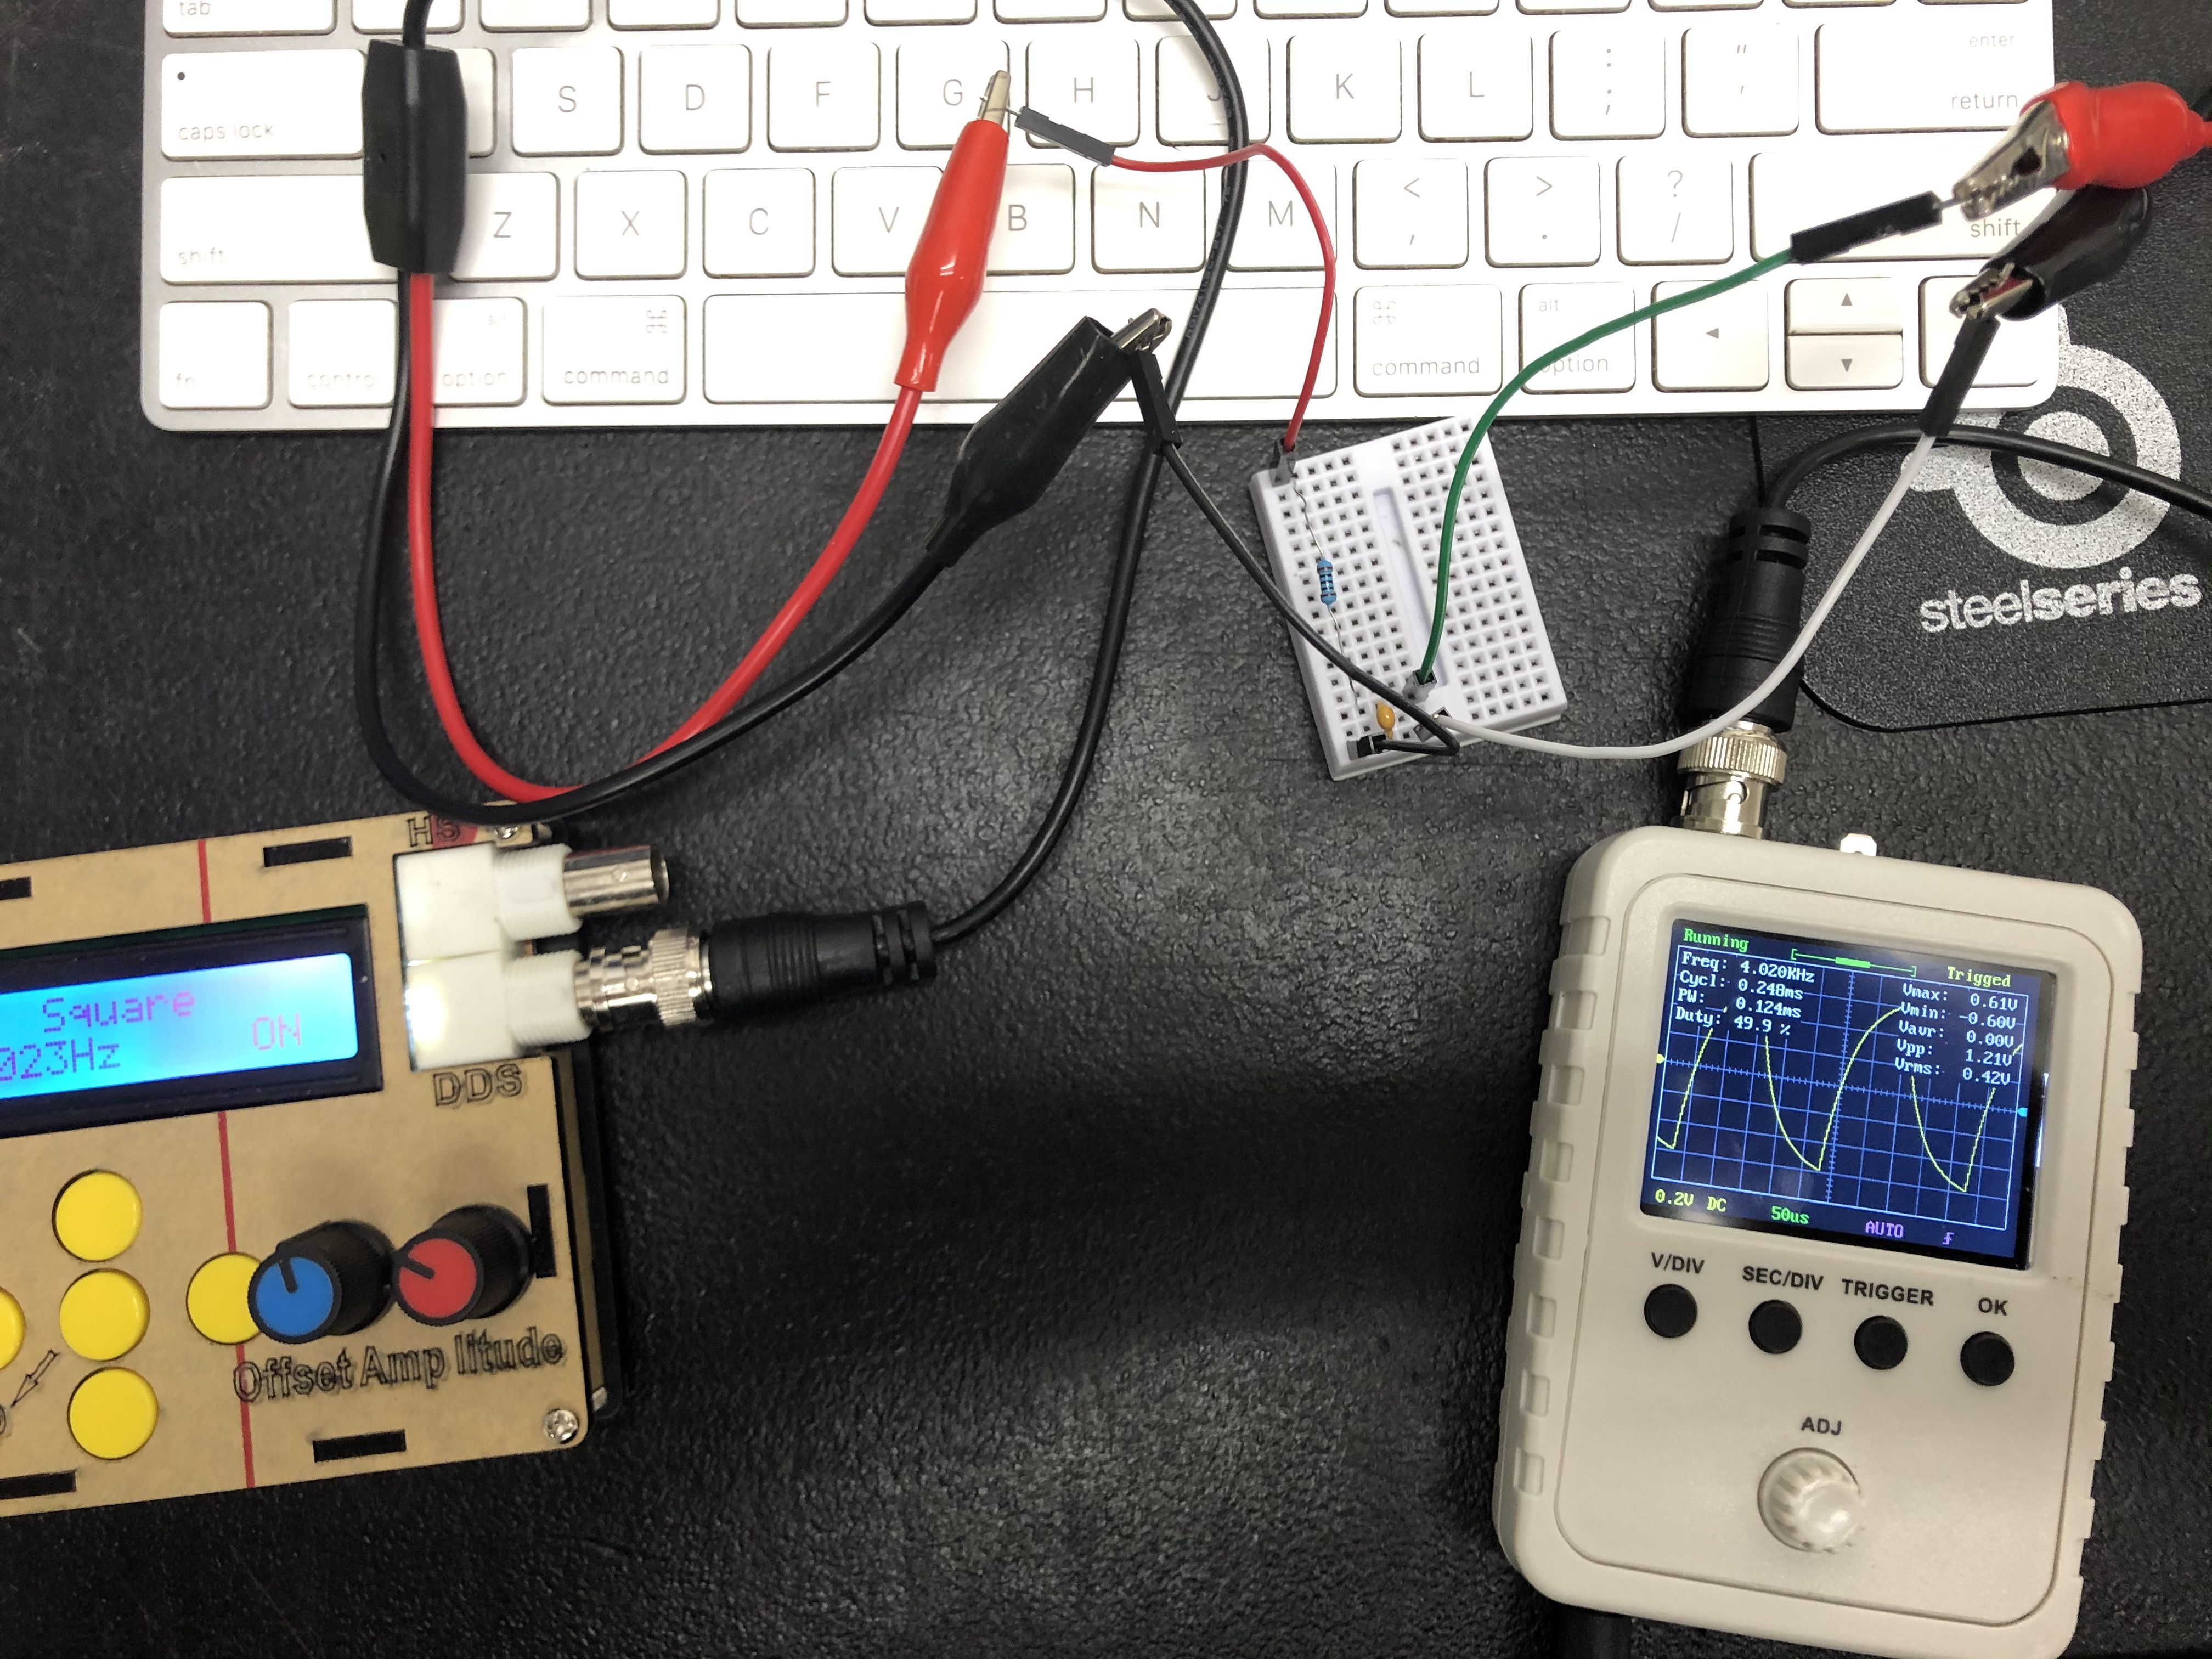
\includegraphics[scale=0.066]{setup1.jpeg}
\end{center}
\begin{center}
  \subsection*{Graph 1}
  % 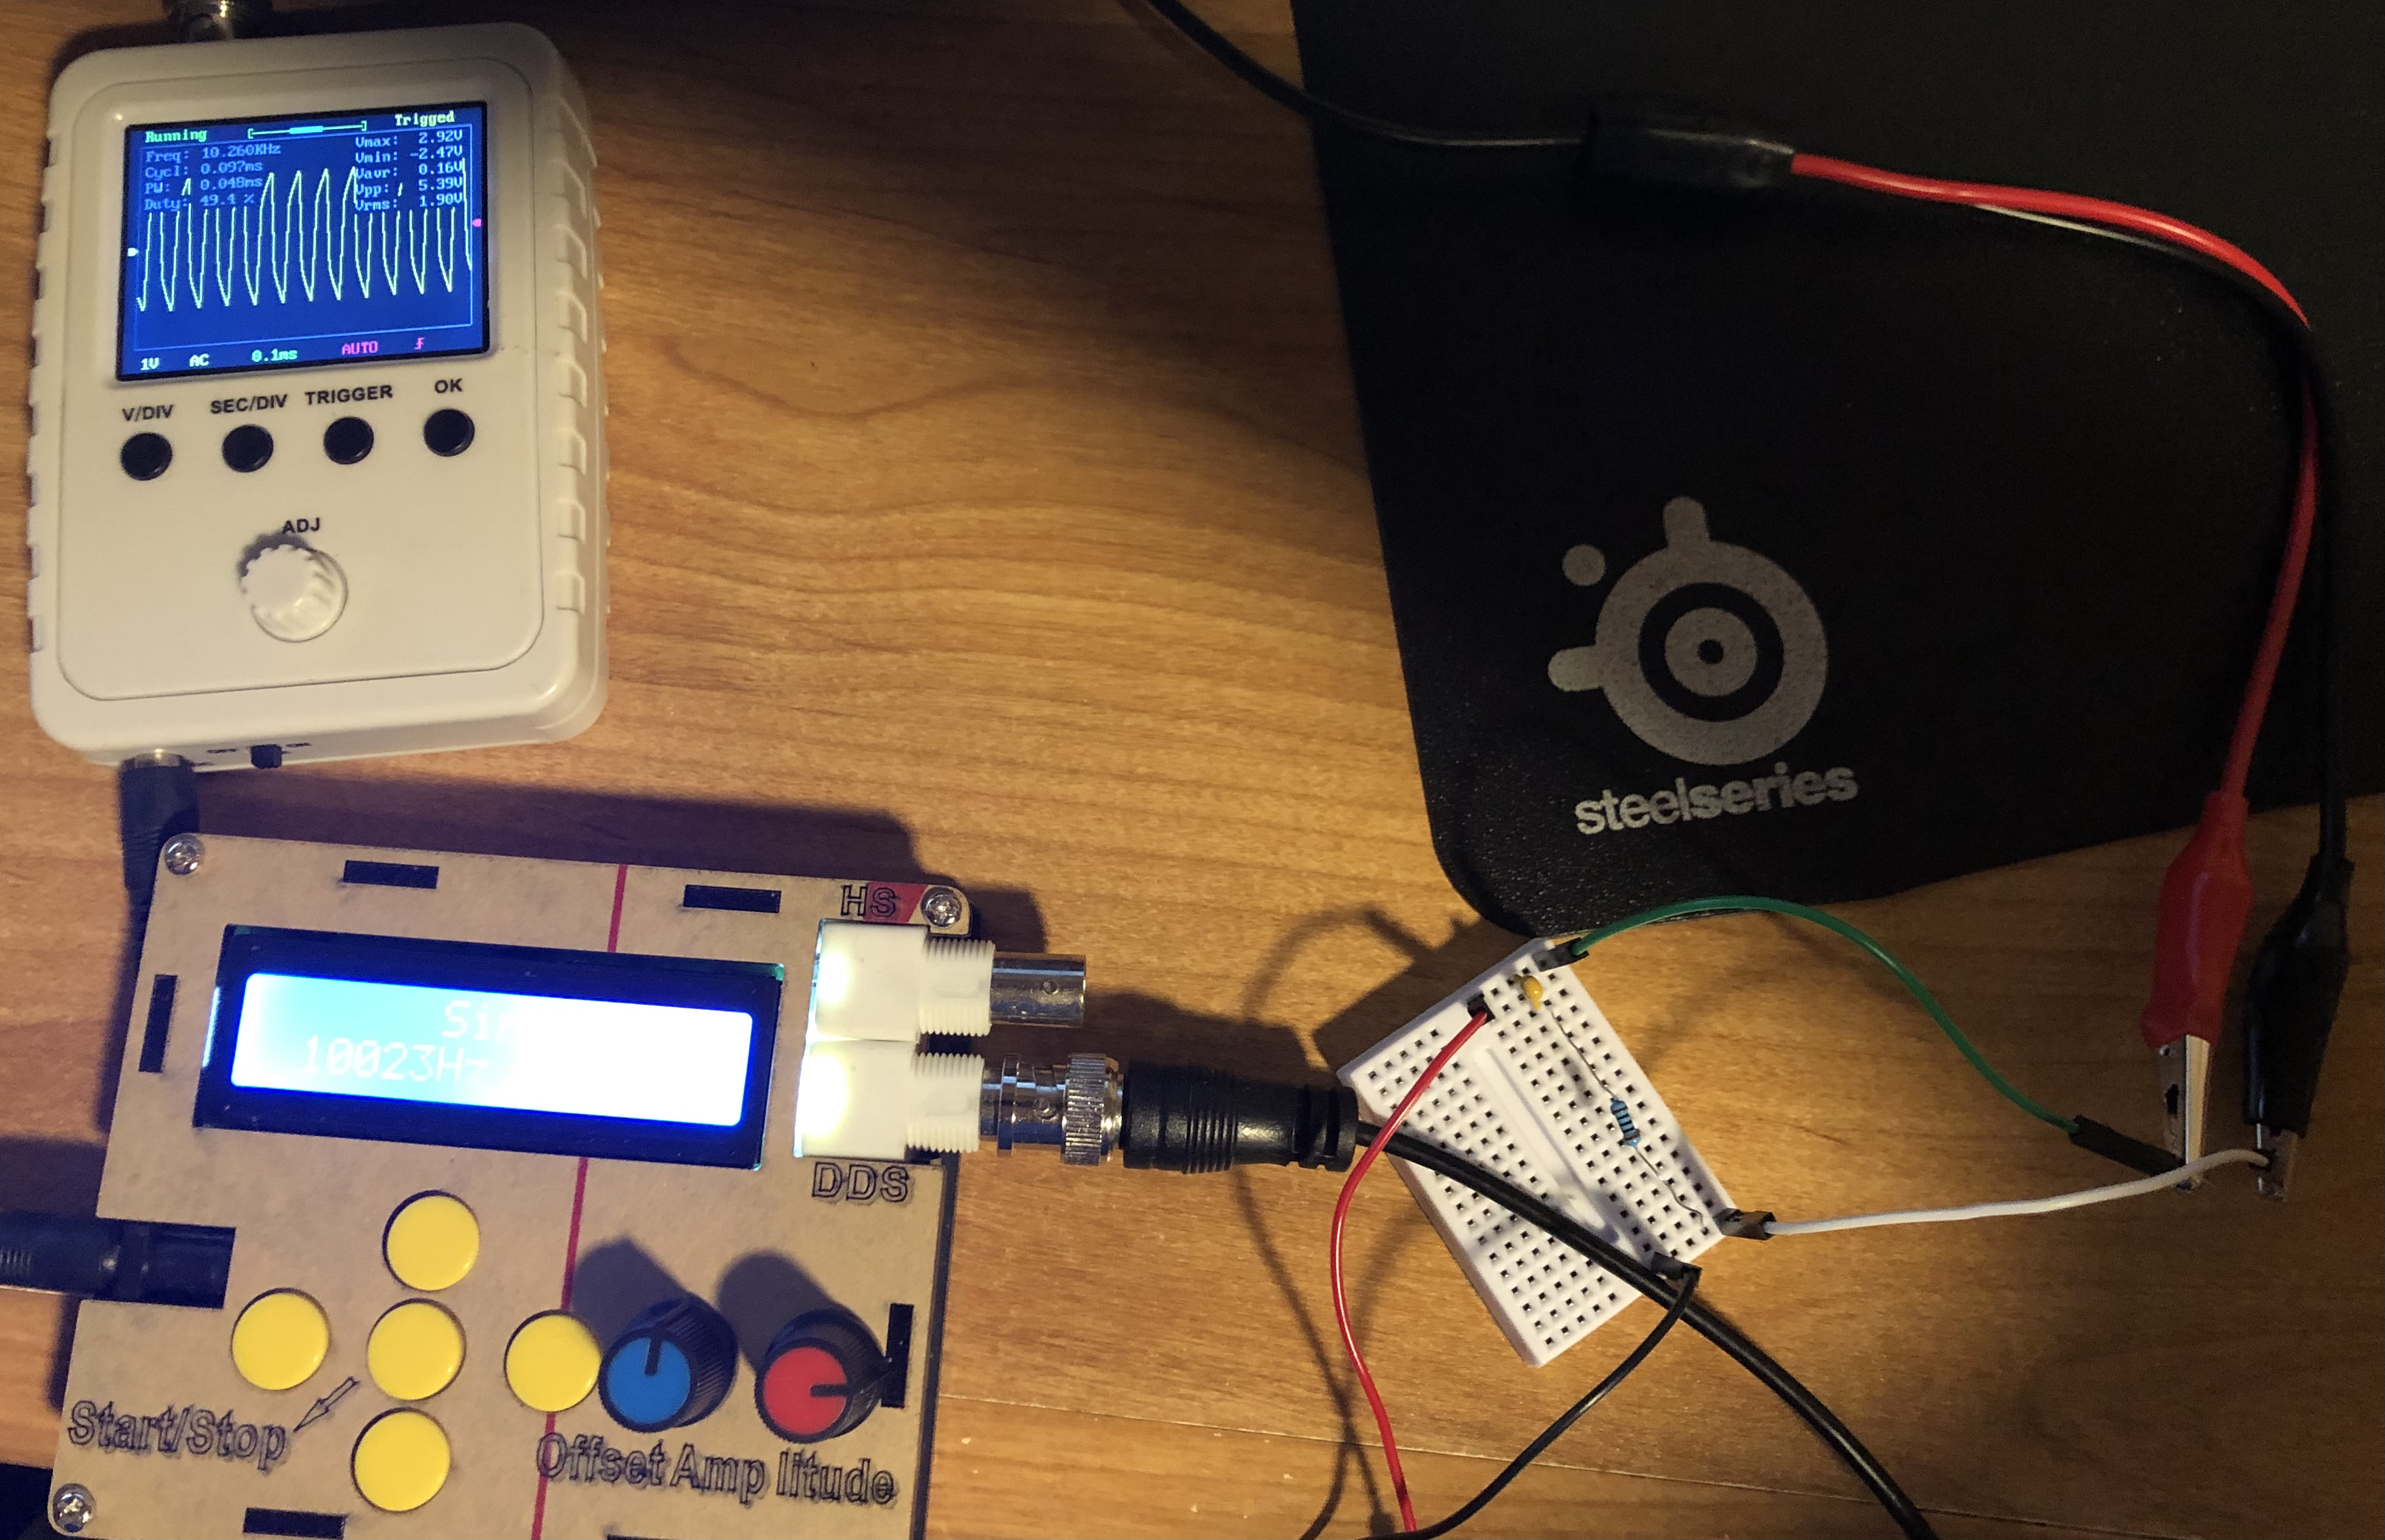
\includegraphics[scale=0.066]{Vrc.jpeg}
  graph 1
  \subsection*{Graph 2}
  % 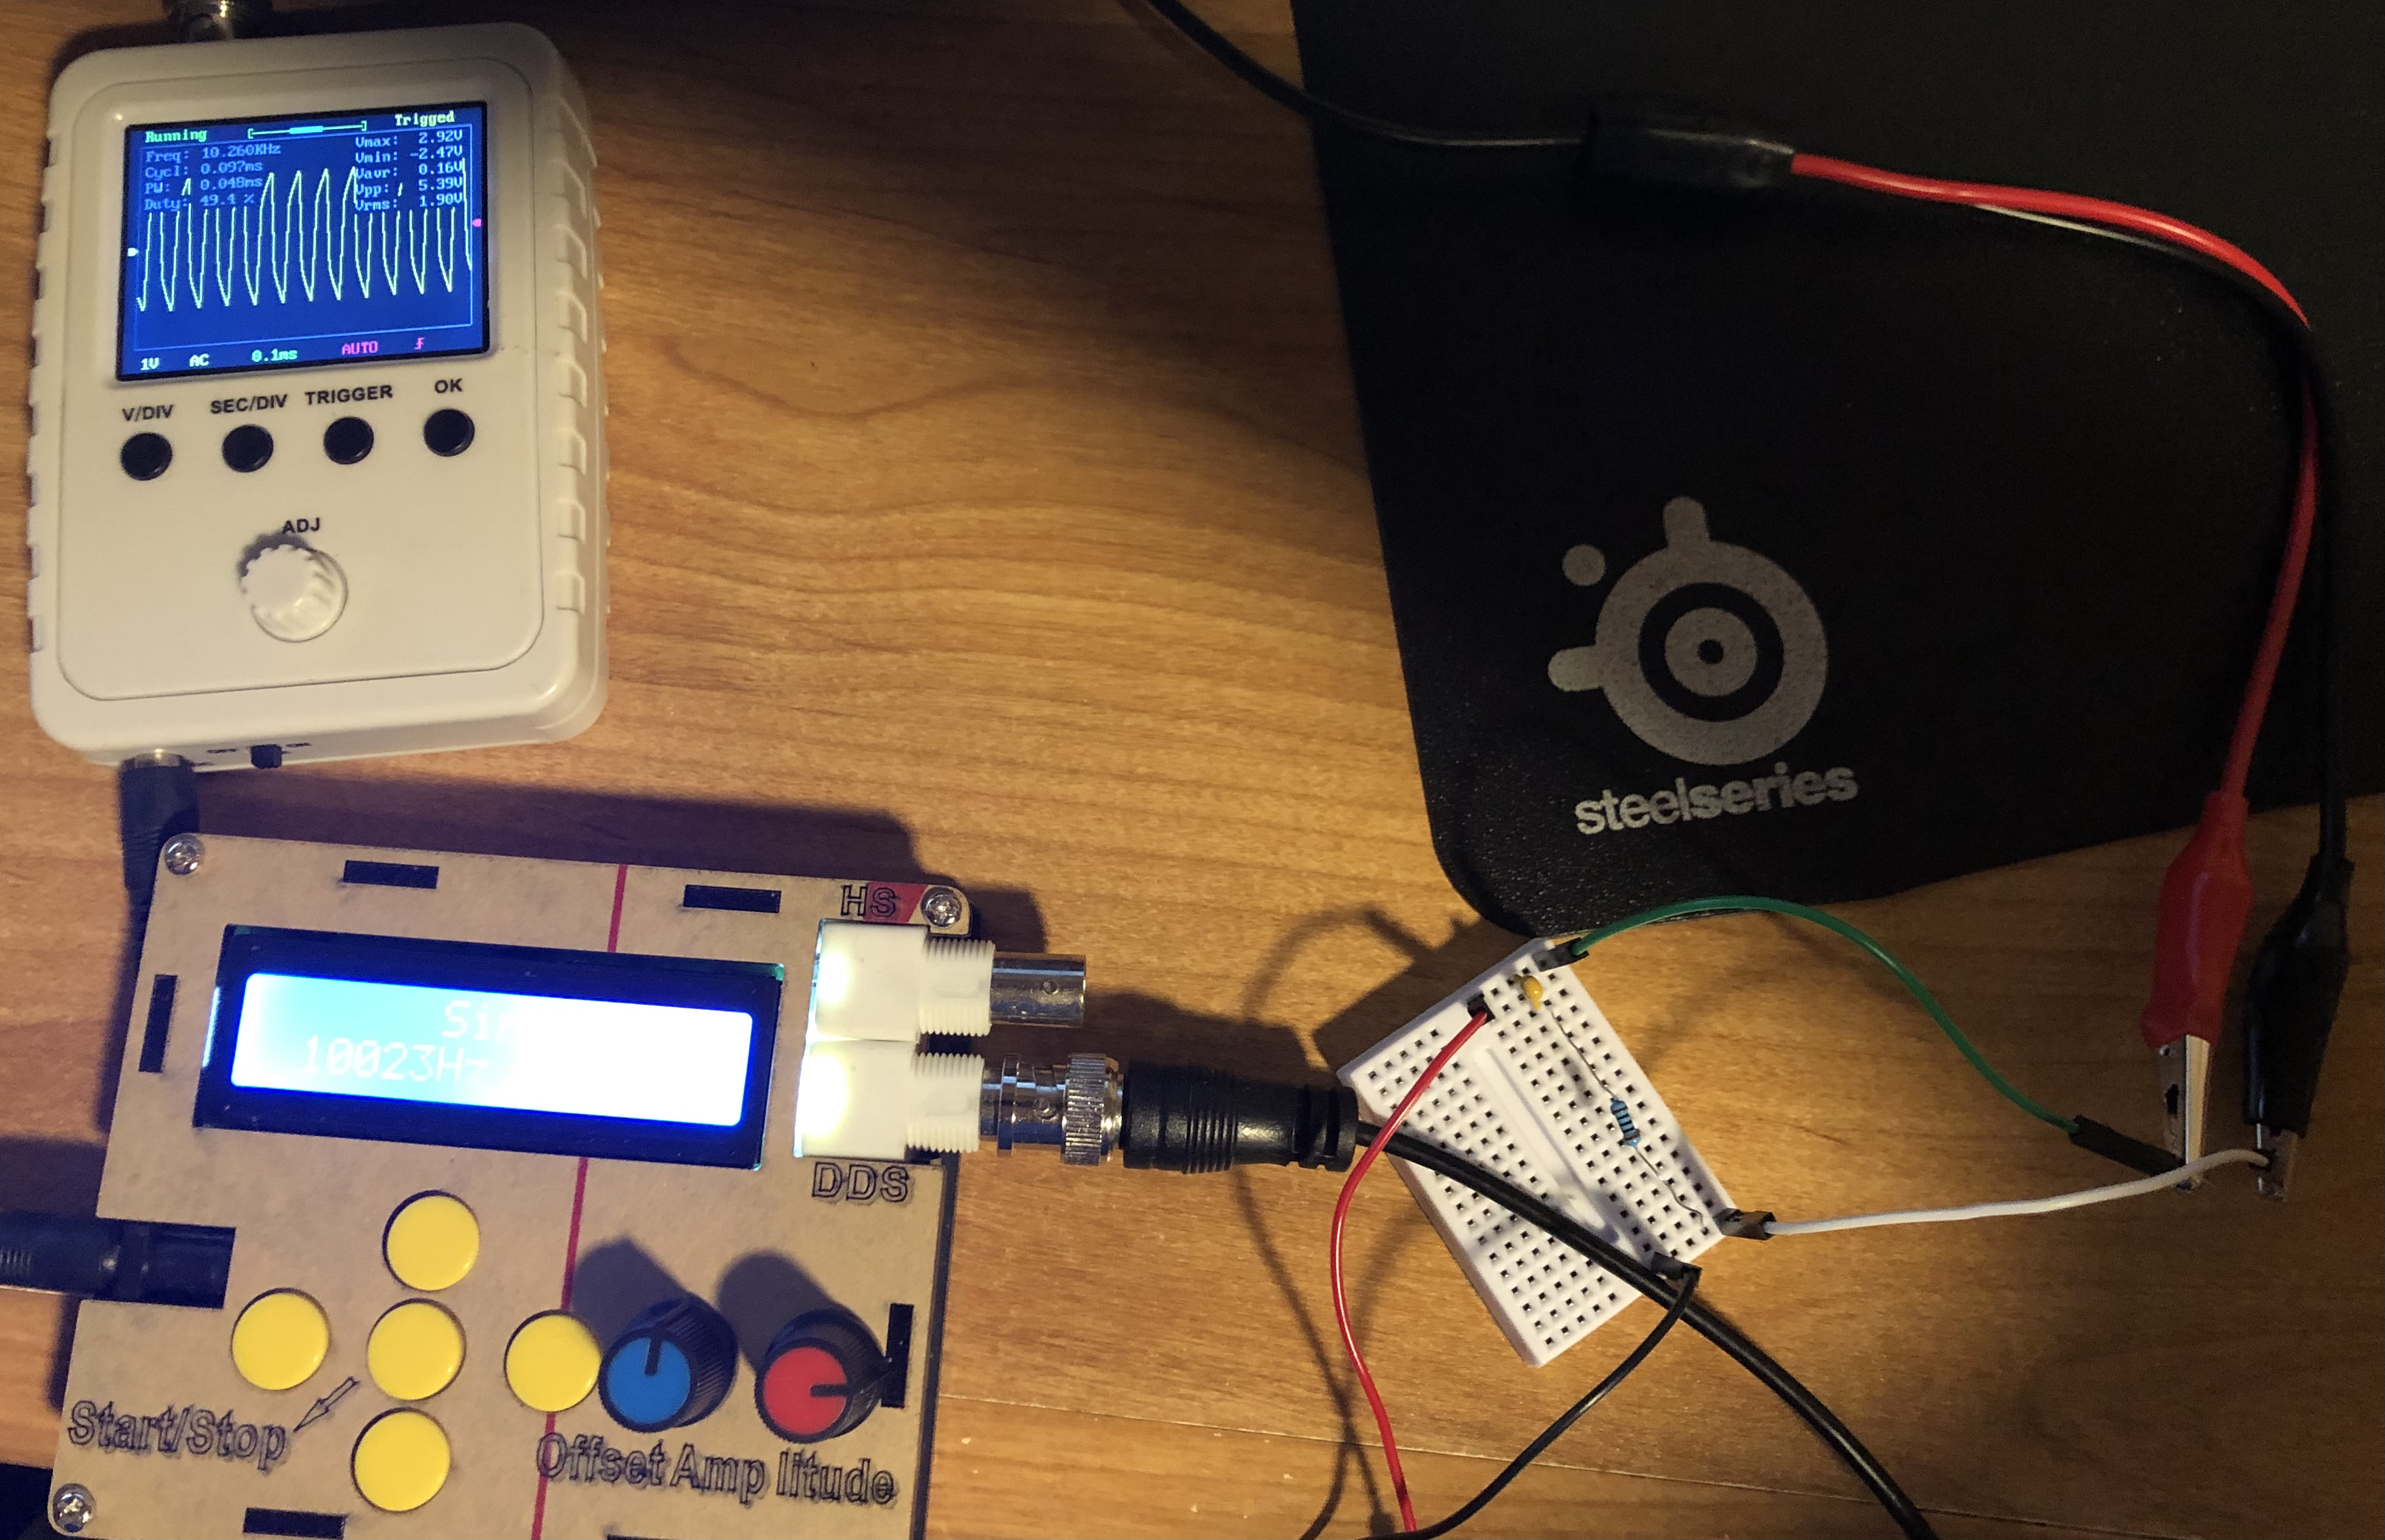
\includegraphics[scale=0.066]{Vrc.jpeg}
  graph 2
\end{center}
\begin{itemize}
  \item What is the value of the slope in the second graph and how does that compare to what you expected?
\end{itemize}
\end{document}
